\section{Environnement}

%%%%%%%%%%%%%%%%%%%%%%%%%%%
%  Environnement          %
%%%%%%%%%%%%%%%%%%%%%%%%%%%

\begin{frame}[fragile]{Environnement de nos attaques}
  \begin{columns}
    \begin{column}{0.5\textwidth}
      \begin{block}{Qemunet}
        \begin{itemize}
        \item Outil pour créer un réseau virtuel
        \item \url{gitlab.inria.fr/esnard/qemunet}
        \end{itemize}
      \end{block}

      \begin{exampleblock}{3 machines}
        \begin{itemize}
        \item Un client (Alpine)
        \item Un serveur (Debian)
        \item Un attaquant (Debian)
        \end{itemize}
      \end{exampleblock}

      \begin{exampleblock}{Lancement de l'attaque SSLStrip}
        \verb+./qemunet/qemunet.sh -x -S sslstrip+

      \end{exampleblock}

    \end{column}

    \begin{column}{0.5\textwidth}
      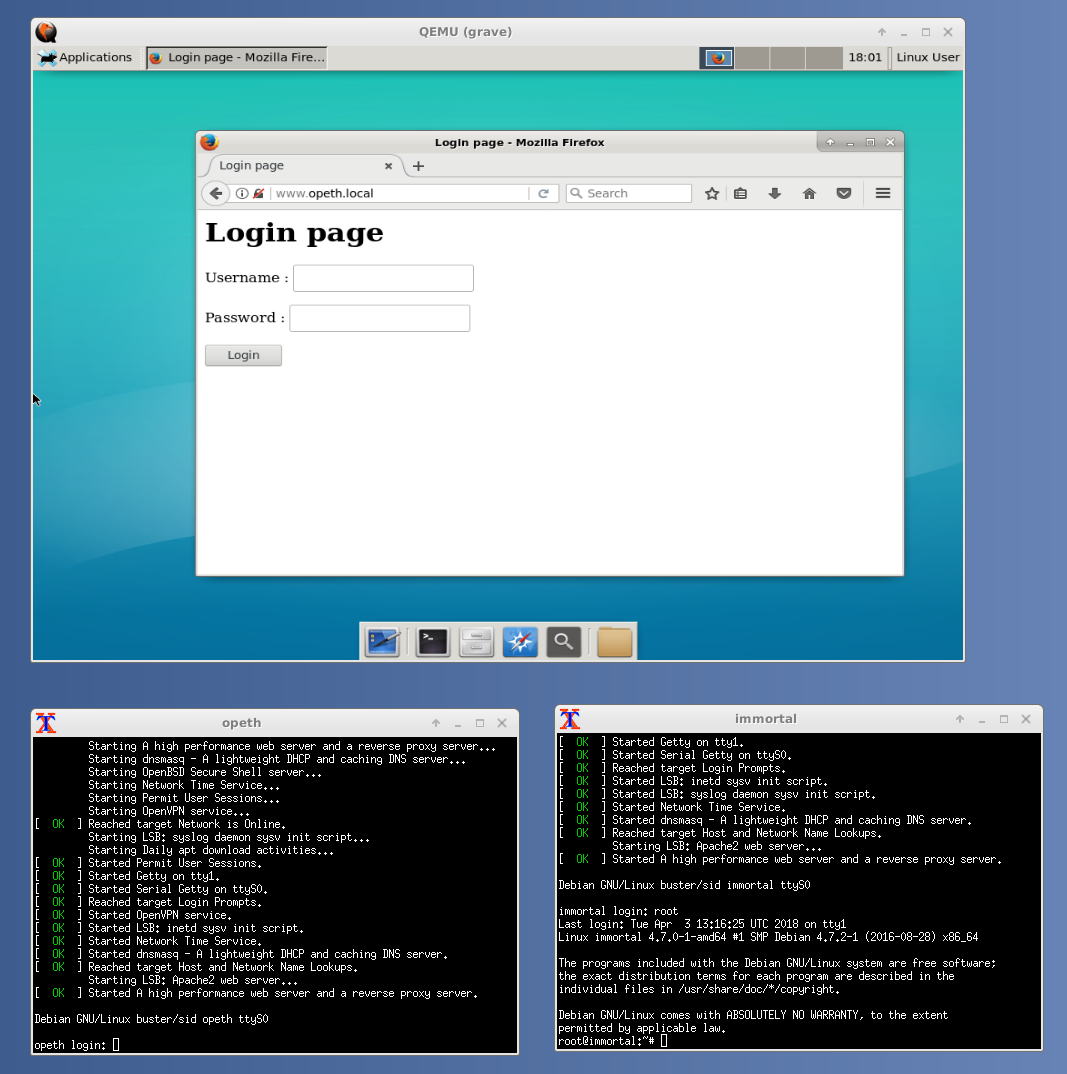
\includegraphics[width=\linewidth]{../medias/qemunet.png}
    \end{column}
  \end{columns}

\end{frame}

%%%%%%%%%%%%%%%%%%%%%%%%%%%
%  Topologie              %
%%%%%%%%%%%%%%%%%%%%%%%%%%%

\begin{frame}{Topologie}
    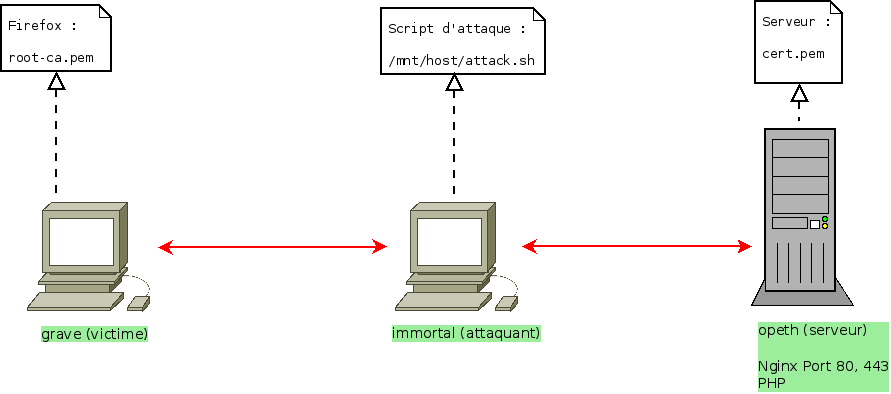
\includegraphics[width=\linewidth]{../medias/topology.png}
\end{frame}
